% To combine into a pdf:
%
% > for x in *.eps; do epstopdf $x; done
% > pdflatex two_leptons.tex
% > acroread two_leptons.pdf
%
% or if you're a tcsh user, replace the for loop with something like this:
% > foreach x (*.eps)
% foreach? epstopdf $x
% foreach? end
%
% or do them all by hand.

\documentclass[landscape]{article}
\usepackage[pdftex]{graphicx}
\pagestyle{empty}
\oddsidemargin  -0.5 in
\evensidemargin -0.5 in
\headheight     0 in
\topmargin      -1 in
\textheight     7.7 in
\textwidth      10 in
\begin{document}
\LARGE
\renewcommand{\labelitemi}{-}
\setlength{\parindent}{0 cm}

\begin{center} \begin{tabular}{p{\textheight} p{4 cm}}
    \begin{minipage}{\linewidth}
      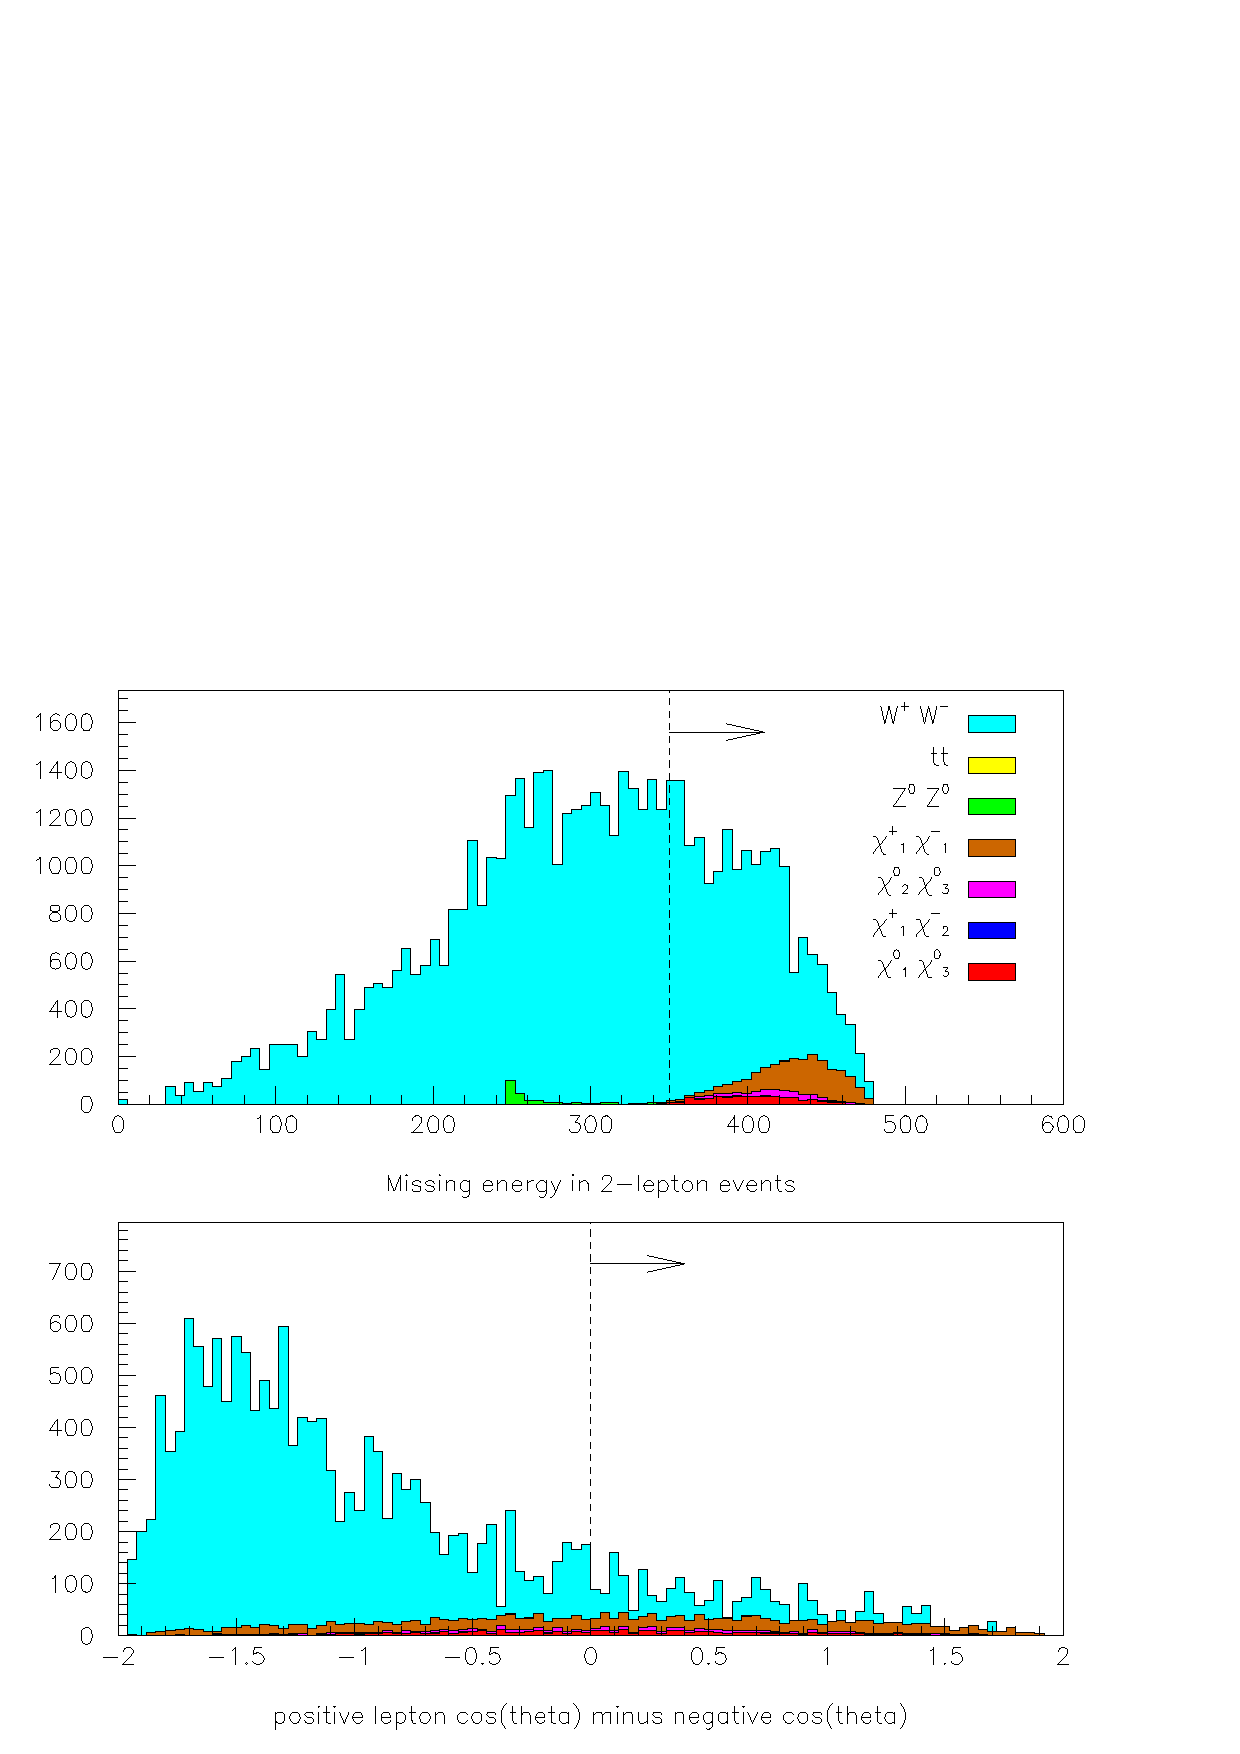
\includegraphics[width=\linewidth]{two_leptons_1.pdf}
    \end{minipage} &
    \begin{minipage}{\linewidth}
      Signal: \\
      \includegraphics[width=\linewidth]{two_leptons_signal.pdf}

      \vspace{1 cm}
      Background: \\
      \includegraphics[width=\linewidth]{two_leptons_background.pdf}

      \vspace{1 cm}
      Background: \\
      \includegraphics[width=\linewidth]{two_leptons_background2.pdf}
    \end{minipage}
  \end{tabular}
\end{center}
\pagebreak

\begin{center} \begin{tabular}{p{\textheight} p{4 cm}}
    \begin{minipage}{\linewidth}
      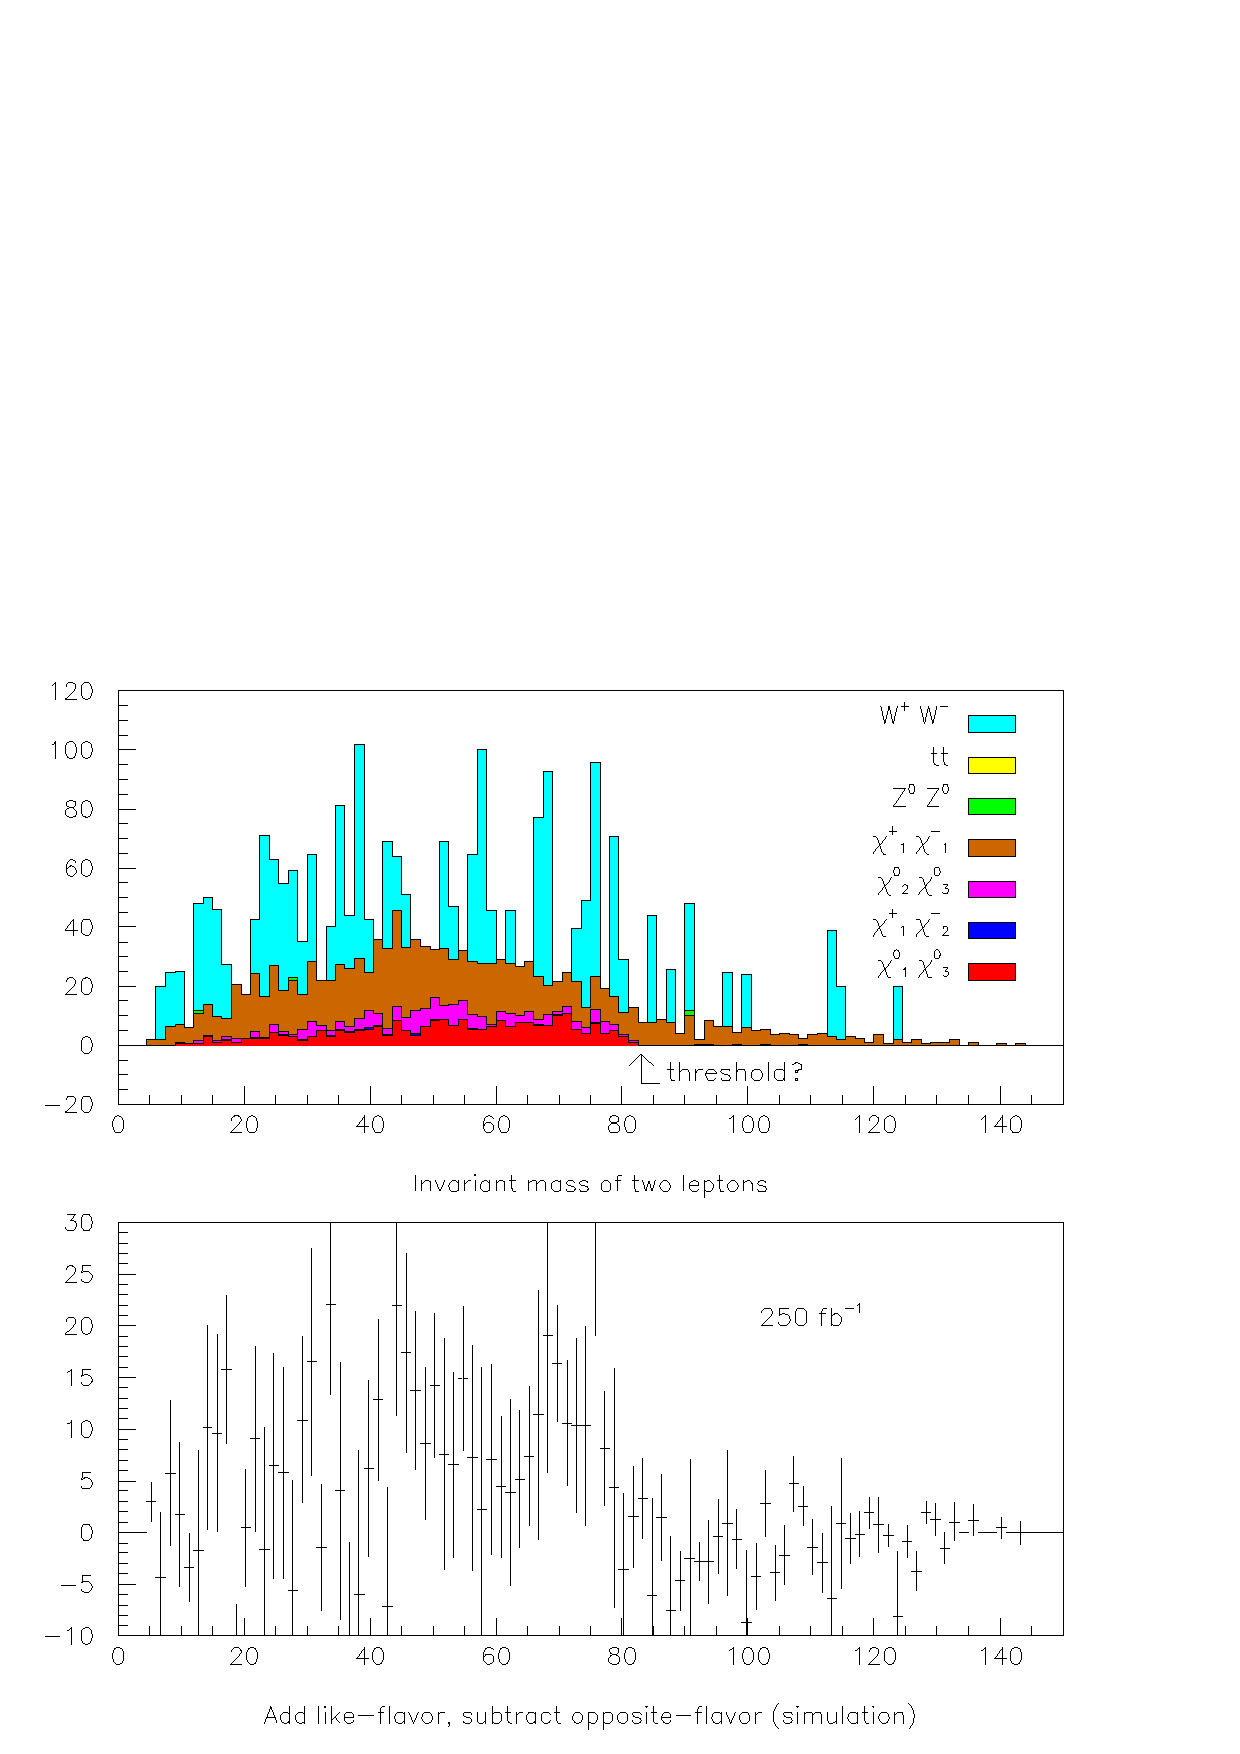
\includegraphics[width=\linewidth]{two_leptons_2.pdf}
    \end{minipage} \hspace{-0.5 cm} &
    \begin{minipage}{4.5 cm}
      Signal always decays into same-flavor leptons

      \vspace{1 cm}
      Backgrounds are 50\% same-flavor, 50\% opposite.

      \vspace{1 cm}
      Another signal:
      \includegraphics[width=\linewidth]{two_leptons_signal2.pdf}
    \end{minipage}
  \end{tabular}
\end{center}

\end{document}
